\chapterOrPart{Discussion}\label{ch:discussion}

\begin{explanation}
    It is mandatory to discuss the obtained results. But it must not necessarily be done in a separate chapter. It can also be part of the chapter with results.
    
    Feel free to alter the name of the chapter and/or the sections.
\end{explanation}

\section{Adaptation Insight}
\label{sec:adaptationInsight}

The results of \Cref{ch:results} reframe the residential demand problem. The executed climate-only cases show declining heating pressure and rising cooling pressure, while the hourly design-year cases show that electrification, not climate forcing alone, dominates peak grid import. Adaptation is therefore treated here as a set of directions supported by the modelled patterns because active cooling final energy is not included, and the investment outputs use illustrative tariff, emission-factor, CAPEX, and O\&M assumptions.


\subsection{Combined Heating/Cooling Service}
\label{sec:adaptation_reversible_hp}

The rise in CDD$_{22}$ from about $14.3$ to $109.3\,^{\circ}\mathrm{C}\cdot\mathrm{d}$ per year under long-term RCP\,8.5 (\Cref{tab:climate_degree_days_results}) makes cooling service a relevant adaptation dimension. The current model does not simulate active cooling electricity, so reversible heat pumps cannot be evaluated as a fully modelled cooling technology. Instead, the investment-adaptation layer reports a service proxy: it combines the cooling-pressure indicator with the technology option’s ability to provide reversible cooling.

\subsubsection*{Reversible-heat-pump adaptation}
\Cref{fig:reversible_hp_adaptation_proxy} should therefore be read as a prioritisation proxy, not as an economic proof that reversible heat pumps outperform heating-only heat pumps. In the current tariff and CAPEX assumptions, the reversible option carries additional annualized cost relative to the air-water heating-only option because the bill ledger does not yet monetize cooling comfort. Its value in this chapter is more specific: it identifies where the heating-to-cooling transition makes a cooling-capable heat-pump configuration the relevant adaptation option to test in the next model version.

\begin{figure}[ht]
  \centering
  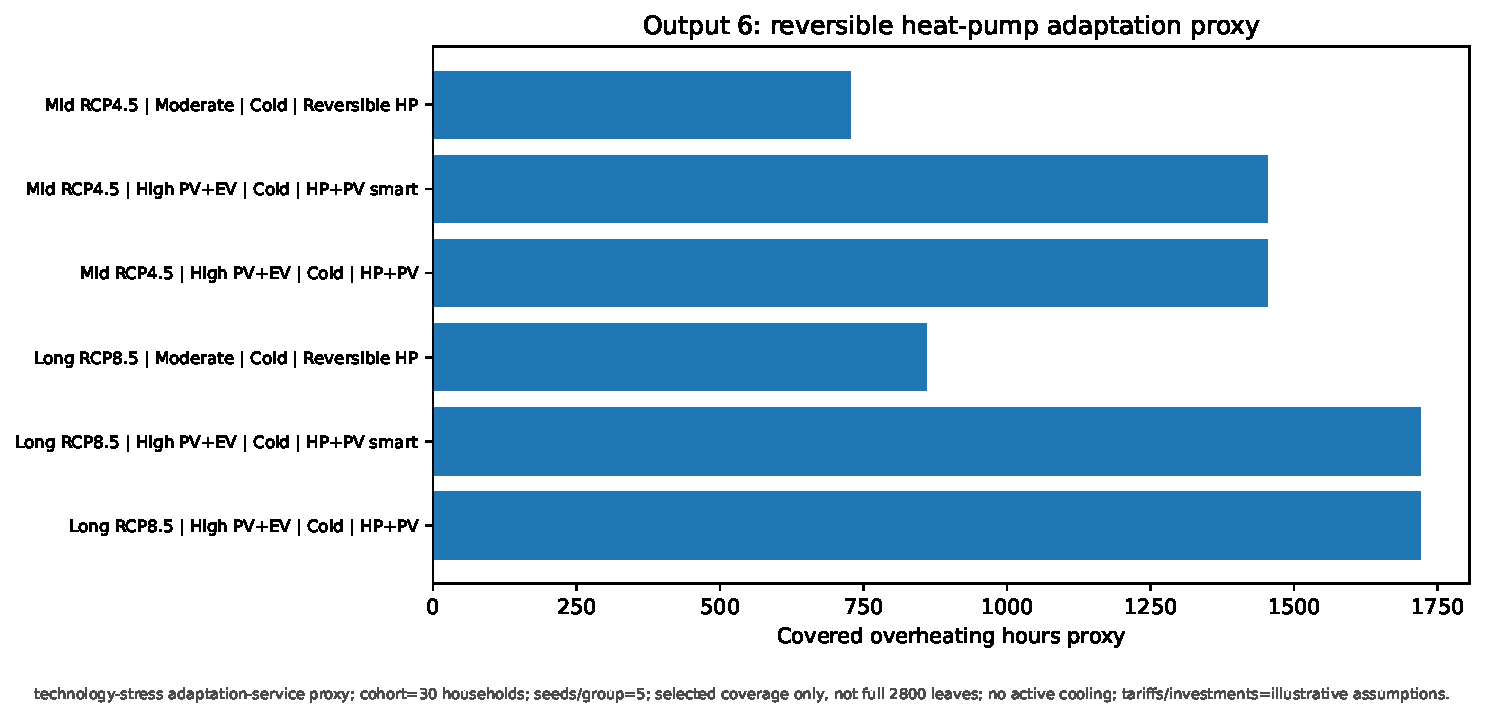
\includegraphics[width=0.9\textwidth]{figures/output6_reversible_hp_adaptation_proxy.pdf}
  \caption{Reversible-heat-pump adaptation-service proxy. The proxy is based on cooling-exposure indicators and technology service capability.}
  \label{fig:reversible_hp_adaptation_proxy}
\end{figure}


\subsection{PV Adaptation}
\label{sec:adaptation_pv_self_consumption}

PV adaptation is interpreted through self-consumption rather than installed capacity alone. \Cref{fig:pv_scr_ssr} reports the PV self-consumption ratio (SCR) and self-sufficiency ratio (SSR) for the executed design-year scenarios, where:
\begin{equation}
    \text{SCR} = \frac{E_\text{PV,self-consumed}}{E_\text{PV,total}}, 
    \quad 
    \text{SSR} = \frac{E_\text{PV,self-consumed}}{E_\text{load,total}}
\end{equation}
The high-electrification PV--EV case raises SCR because heat-pump and EV loads absorb a larger fraction of local generation. In the cold-design long-term RCP\,8.5 case, SCR rises from about $0.37$ under frozen stock to about $0.48$ under moderate electrification and $0.62$ under the high-electrification PV--EV case.

\subsubsection*{PV Self-consumption limitations}
\Cref{fig:pv_scr_ssr} also shows the limitation. SSR remains very low in the electrified cases because the electrified load is much larger than the modelled PV generation. PV therefore improves local use of generated electricity, but in the current scenario set it does not remove the peak-grid problem identified in \Cref{sec:systemImpact}. Under low or zero export value, this makes self-consumption timing more important than export credit; it does not make the high-electrification case economically favourable under the current post-processing assumptions.

\begin{figure}[ht]
  \centering
  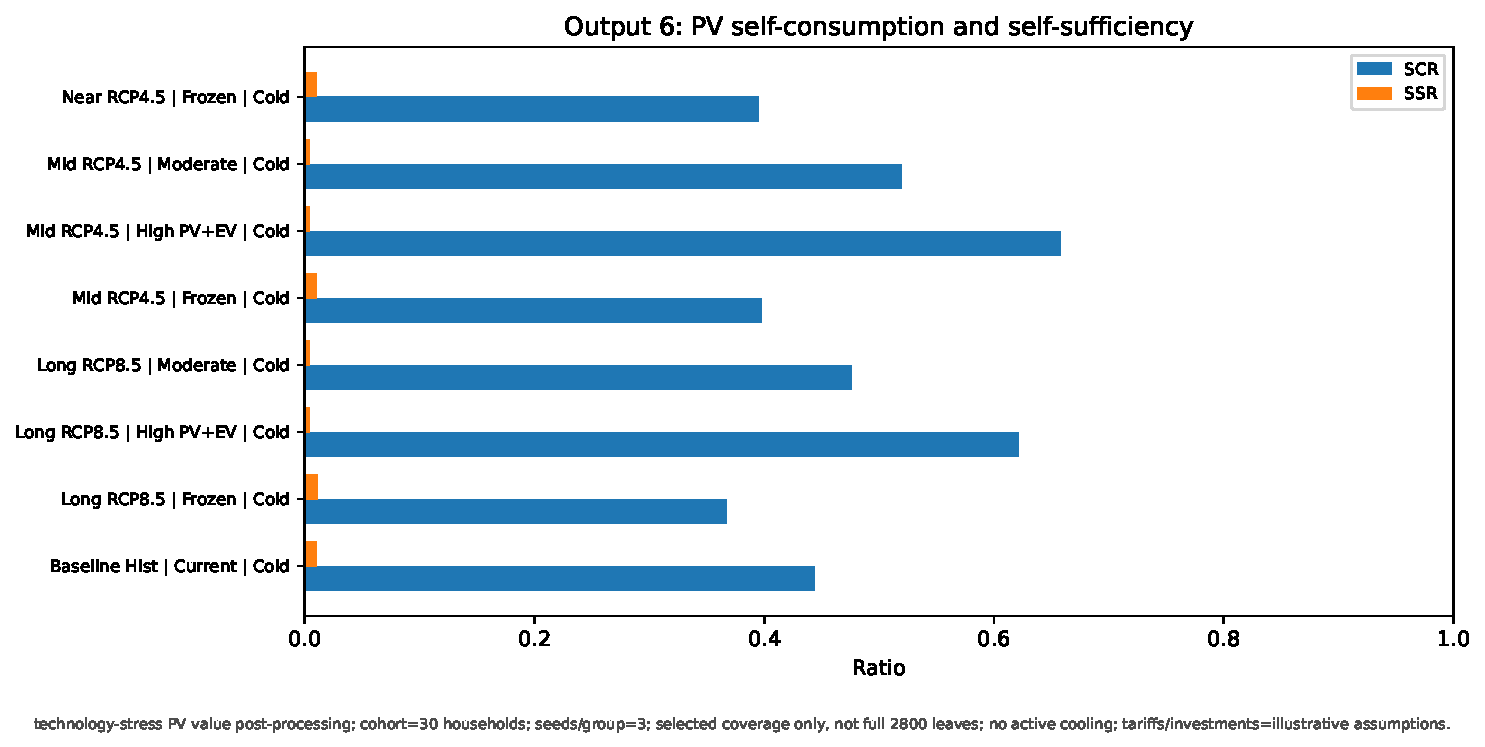
\includegraphics[width=0.9\textwidth]{figures/output6_pv_scr_ssr.pdf}
  \caption{PV self-consumption ratio and self-sufficiency ratio across executed technology cases.}
  \label{fig:pv_scr_ssr}
\end{figure}


\subsection{Residential Electrification}
%% Impact based on outputs of results chapter, good/bad, why, money-wise, etc. %%
The results complicate a simple pro-electrification interpretation. In the climate-only comparison, warming reduces heating pressure under a frozen residential stock: the long-term RCP\,8.5 case reduces HDD$_{18}$ by about \SI{31}{\percent} and useful-heating demand by about \SI{33}{\percent}. However, this physical reduction does not translate into a major reduction in residential grid stress, because the frozen-stock case remains largely gas-dominated. The hourly design-year results show that the dominant system change is instead the technology transition itself.

Under the executed long-term RCP\,8.5 cold-design-year case, frozen stock leaves peak grid import almost unchanged relative to the historical baseline, while moderate electrification raises the cohort peak to about \SI{87}{kW} and the high-electrification PV--EV case raises it to about \SI{184}{kW}. This means that residential electrification is not merely a fuel-substitution problem; it is also a coincidence and infrastructure problem. The modelled peak increase is much larger than the climate-only peak effect in the executed scenario subset.

The economic and emissions outputs point in the same direction of conditionality. Moderate electrification reduces operational emissions under the fixed electricity-emission factor, but it raises annual bills and annualized costs under the current tariff and CAPEX assumptions. The high-electrification PV--EV case performs worse in the current accounting: PV raises self-consumption, but the electrified load is large enough that grid import remains dominant, and operational emissions increase under the fixed-factor assumption. These results should not be read as evidence against electrification in general. Rather, they show that electrification is only beneficial under the right accompanying system conditions: lower-carbon electricity, sufficient network capacity, flexible heat-pump and EV operation, tariff structures that reward useful flexibility, and PV deployment that prioritises self-consumption rather than export.

The main discussion implication is therefore that electrification is a necessary decarbonisation pathway but not an automatically benign residential-demand pathway. In this model, unmanaged electrification shifts the residential challenge from annual heating demand toward peak power, coincidence, and tariff-sensitive affordability. The adaptation question is consequently not whether electrification occurs, but how it is coordinated with grid planning, cooling demand, PV self-consumption, and demand-side flexibility.



\subsection{From Stress to Strategy}
\label{sec:adaptation_summary}

Three implications follow from the executed results. First, climate forcing alone reduces heating demand and raises cooling pressure, but it does not materially increase the observed residential grid peak with the frozen stock. Electrification does: the hourly design-year results raise the cohort peak by roughly five to ten times relative to the historical current-stock baseline.

Second, cooling pressure is real in the indicator space but incomplete in the energy ledger. A future active-cooling module is needed before the model can quantify summer electricity demand, peak timing shifts, or the interaction between cooling load and PV generation.

Third, the economic and emissions results are conditional on tariff, export-credit, CAPEX, O\&M, and fixed electricity-emission assumptions. The defensible adaptation message is therefore about system shape rather than precise welfare ranking: electrification creates the dominant grid-stress channel; cooling-capable heat pumps become relevant because cooling pressure rises; and PV value depends increasingly on local absorption rather than export.

\begin{quote}\itshape
Under one CORDEX chain and the configured Belgian baseline, residential electrification is the dominant source of peak grid stress in the executed future design-year cases. Climate forcing alone is secondary for grid peak under the frozen stock, while rising cooling pressure and low-export PV economics make reversible heat-pump service and PV self-consumption the key adaptation directions to evaluate further.
\end{quote}


\pagebreak
\section{Limitations}\label{sec:limitations}

The limitations of this work are primarily ones of evidential scope. The model
supports comparison of internally consistent climate--technology scenarios, but
several components are not strong enough for national forecasting,
distribution-network design, or precise household-level prediction.


\subsection{Executed Scenario Coverage}
\label{sec:limitationsScenarioCoverage}

The scenario-tree design defines a far larger factorial space than was executed. The thesis evidence uses the completed subset in the canonical artefacts: 37 full-window climate/annual-demand leaves from \texttt{scenario\_tree/} and 48 hourly design-year leaves from \texttt{output34/}, i.e.\ 85 of the planned 2800 leaves.

The two sets answer different questions. The full-window runs drive the annual climate-pressure and heating-demand comparisons across climate windows and RCP pathways; the \texttt{output34} runs drive the hourly peak, diversity, bill, emissions, and adaptation diagnostics, but only for selected climate--technology combinations and a smaller cohort. The chapter accordingly makes no claim to full factorial coverage across pathway, window, technology case, design year, and seed.


\subsection{Climate Forcing Limitations}
\label{sec:limitationsClimateForcing}

The CORDEX forcing in the scenario tree is daily rather than hourly. Temperature and surface shortwave radiation are processed as daily variables, and the hourly
\texttt{output34} workflow forward-fills them to the model timestep. Hourly variation in those runs therefore arises from stochastic demand, occupancy, appliances, DHW, EV charging, PV profiles, and heating control, rather than from a reconstructed hourly future-weather signal.

Future-climate results are consequently most defensible at daily, seasonal, annual, and scenario-comparison scales, and should not be read as precise simulations of future hourly weather extremes, intra-day heat-wave dynamics, or sub-daily solar variability. The evidence also rests on a single CORDEX chain and a nearest-point extraction around the Belgian target location, rather than a multi-model ensemble or a spatially aggregated climate field; inter-GCM/RCM uncertainty, bias-correction uncertainty, and local urban or microclimate effects lie outside it.


\subsection{Demand Model \& Empirical Validation}
\label{sec:limitationsValidation}

The demand model combines archetype, stock, stochastic-use, and technology assumptions---appropriate for scenario exploration, but not equivalent to calibration against a large sample of measured Belgian household load curves. The clearest external warning is the Fluvius aggregate validation, where the representative-profile comparison currently fails: CVRMSE around 88\%, Pearson correlation around 0.40, annual-energy error around 56\%, and peak-timing error around 18 hours. This bounds any claim to reproduce observed Belgian aggregate electricity profiles.
\newline The remaining validation layers are more supportive but narrower. The Richardson-style comparison speaks to stochastic diversity structure rather than Belgian empirical accuracy; the KU\,Leuven high-frequency check covers only three houses and cannot provide statistical validation. PV validation is strong against PVGIS and Elia at physical and national-profile level but only moderate against the Fluvius residential PV signature. EV timing matches the Fluvius-derived signature well, while the base annual home-charging magnitude sits roughly 43\% below the reference---a gap the calibration sensitivity attributes to the annual-energy assumption rather than to timing.


\subsection{Cooling \& Comfort Scope}
\label{sec:limitationsCooling}

The model reports cooling pressure through indicators such as $\text{CDD}_{22}$, overheating exposure, indoor-temperature exceedance, and adaptation proxies, but the executed scenario-tree outputs contain no active cooling final electricity demand. The rise in cooling pressure under warmer scenarios is therefore visible as a climate and comfort signal that is not yet converted into summer electricity demand, cooling peak load, or cooling-related bills and emissions.

The reversible-heat-pump adaptation result should accordingly be read as a service and planning proxy: it shows that cooling-capable heat pumps gain relevance as heating demand falls and cooling pressure rises, without establishing a monetised investment optimum or simulating active cooling operation.


\subsection{Techno-Economic Limitations}
\label{sec:limitationsTechnoEconomic}

The technology cases are scenario assumptions rather than adoption forecasts. They support comparison of frozen-stock, moderate-electrification, and high-electrification futures, but do not model how households actually choose technologies, renovate, or adopt EVs and PV.
\newline Grid stress is captured through cohort-level grid-import peaks and threshold exceedance, with no distribution-network power-flow model. The results thus locate demand-side peak pressure without resolving transformer loading, voltage violations, cable congestion, protection constraints, or feeder-specific hosting capacity.

The bill figures are post-processing under configured tariff assumptions and are best read as illustrative tariff scenarios rather than Belgian tariff forecasts. The emissions figures are operational and factor-based: they apply fixed emission factors, exclude embodied emissions, omit time-varying marginal electricity factors, and give no export credit for displaced system emissions. These assumptions suffice for comparing directions within the model, but not for final policy-costing or lifecycle-carbon claims.


\subsection{Overall Interpretation Boundary}
\label{sec:limitationsInterpretationBoundary}

The model is strongest for comparing internally consistent scenario directions:
the reduction in heating pressure under warming, the dominance of electrification
in the hourly peak signal, the tariff sensitivity of household bills, and the
conditional nature of operational-emissions reductions. It is weaker as a source
of absolute national figures, and the results are best read as a structured
scenario experiment for Belgian residential demand rather than a calibrated
national energy-system forecast.


\pagebreak
\section{Future Work}\label{sec:futurework}

Future work should focus on turning the present scenario framework into a more
complete empirical and operational platform, prioritising the gaps identified in
\Cref{sec:limitations}.


\subsection{Scenario Tree Broadening}
\label{sec:futureworkScenarioTree}

The first priority is to execute a larger and more balanced share of the planned
tree, extending the hourly \texttt{output34} workflow beyond the selected
design-year and technology combinations so that uncertainty bands can be
reported across climate windows, pathways, technology cases, seeds, and design
years. This also requires a formal link between the full-window annual runs and
the hourly design-year runs---either hourly simulation over longer windows, or a
documented sampling strategy that maps each annual climate window to
representative hourly design years.


\subsection{Climate Forcing \& Cooling Modelling}
\label{sec:futureworkClimateCooling}

The climate pipeline should move from a single CORDEX chain to a multi-model
ensemble, and from a nearest-point extraction to spatial aggregation over
Belgium, so that results report spread across GCM/RCM combinations rather than
one realisation. The hourly treatment of future weather should likewise replace
the forward-filled daily forcing with a documented temporal downscaling of
temperature and solar radiation, or with bias-corrected hourly climate
products---most important for peak-load, cooling, PV, and heat-pump questions.
Cooling should then be implemented as an explicit end use, converting the
present cooling-pressure indicators into summer electricity demand, peak
contribution, comfort, bills, and emissions, which would also make the
reversible-heat-pump adaptation analysis operational.


\subsection{Empirical Validation}
\label{sec:futureworkValidation}

The priority for validation is measured Belgian household or feeder-level
electricity data at sufficient temporal resolution. The failing Fluvius
aggregate comparison should be treated as an open model-development issue and
diagnosed against its likely causes: annual magnitude, appliance profiles,
heating-electrification assumptions, occupancy schedules, profile alignment, or
reference representativeness. Each validation purpose---end-use calibration,
diversity structure, aggregate load shape, PV, EV, and high-frequency event
realism---should also carry its own acceptance criteria, so that strength in one
layer is not overread as validation of another.


\subsection{Electrification \& Flexibility}
\label{sec:futureworkElectrification}

The electrification scenarios should gain an explicit flexibility layer.
Heat-pump preheating, thermal storage, EV smart charging, PV self-consumption,
and tariff-responsive operation are currently represented only partly or through
post-processing sensitivities, and a physical dispatch or control layer would
test whether the large electrification peaks can be reduced without unacceptable
comfort, cost, or emissions penalties. The technology stock should also be tied
to renovation pathways and adoption constraints---heat-pump suitability by
envelope quality, emitter temperature, dwelling type, ownership, and renovation
state---making the scenarios less stylised and more policy-relevant.


\subsection{Distribution-Network \& System Coupling}
\label{sec:futureworkGrid}

The cohort-level import metrics should be connected to a low- or medium-voltage
network model, allowing transformer loading, feeder congestion, voltage
deviations, and hosting capacity to be assessed directly rather than inferred
from demand-side peaks. Coupling the household model to system-level
assumptions---time-varying marginal emission factors, dynamic wholesale prices,
renewable availability, and grid constraints---would further improve the bill
and emissions results, particularly for PV, EV charging, and heat-pump
operation.


\subsection{Economic \& Emissions Accounting}
\label{sec:futureworkEconomicsEmissions}

The bill model should adopt more detailed Belgian tariff structures (supplier
contracts, capacity tariffs, taxes and levies, injection compensation, regional
differences), and the investment layer should move beyond illustrative CAPEX and
O\&M assumptions toward explicit retrofit costs, lifetimes, discount rates, and
affordability constraints. The emissions model should replace fixed operational
factors with time-varying, scenario-dependent ones and, where the scope extends
to lifecycle impact, include embodied emissions for PV, batteries, heat pumps,
EVs, and renovation measures. Exported PV should be accounted for consistently,
whether on a household-boundary or a system-displacement basis.


\subsection{Reproducibility \& Benchmarking}
\label{sec:futureworkReproducibility}

Finally, the manifest-based provenance already attached to each
\texttt{scenario\_leaf\_id} should be extended with automated regression tests on
the headline thesis metrics, so that changes in code, input data, or assumptions
surface as changes in the reported results. This would support both academic
audit and comparison with other residential-demand models.

% Future work should focus on converting the present scenario framework into a more complete empirical and operational modelling platform. 


% \subsection{Complete and Broaden the Scenario Tree}
% \label{sec:futurework_scenario_tree}

% The first priority is to complete a larger share of the planned scenario tree and to make the executed subset more balanced. In particular, the hourly \texttt{output34} workflow should be extended beyond the selected design-year and technology combinations used in this thesis. A fuller run matrix would allow uncertainty bands across climate windows, pathways, technology cases, stochastic seeds, and design years, instead of relying on selected contrasts.

% A second priority is to standardise the connection between the full-window annual runs and the hourly design-year runs. At present, the former are best suited to annual climate-pressure interpretation, while the latter are best suited to peak and techno-economic interpretation. Future work should either run hourly simulations over longer climate windows or define a formal sampling strategy that maps annual climate windows to representative hourly design years.


% \subsection{Improve Climate Forcing and Cooling Modelling}
% \label{sec:futurework_climate_cooling}

% The climate pipeline should be extended from a single CORDEX chain to a multi-model ensemble. This would allow the thesis-style results to report spread across GCM/RCM combinations rather than only one climate realisation. Spatial aggregation over Belgium or over representative Belgian regions would also be preferable to a single nearest-point extraction when making national statements.

% The hourly treatment of future weather should also be improved. Rather than forward-filling daily CORDEX variables to hourly timesteps, future work could apply a documented temporal downscaling method for temperature and solar radiation, or couple the model to bias-corrected hourly climate products where available. This is especially important for peak-load, cooling, PV, and heat-pump performance questions.

% Active cooling should be implemented as an explicit end use. The current model can identify rising cooling pressure, but future work should convert that pressure into cooling electricity demand, summer peak contribution, indoor comfort improvement, bill impacts, and emissions impacts. This would make the reversible-heat-pump adaptation analysis more operational.


% \subsection{Strengthen Empirical Validation}
% \label{sec:futurework_validation}

% The most important validation extension is measured Belgian household or feeder-level electricity data with sufficient temporal resolution and metadata. The current Fluvius aggregate validation fails and should be treated as an open model-development issue. Future work should diagnose whether the failure comes from annual magnitude, appliance profiles, heating electrification assumptions, occupancy schedules, profile alignment, or the representativeness of the reference data.

% Validation should also be separated more sharply by purpose. End-use calibration, stochastic diversity validation, aggregate load-shape validation, PV validation, EV validation, and high-frequency event realism should each have their own acceptance criteria. This would prevent supportive evidence in one layer from being overread as validation of another layer.


% \subsection{Extend Electrification and Flexibility Modelling}
% \label{sec:futurework_electrification}

% The electrification scenarios should be expanded with explicit flexibility. Heat-pump preheating, thermal storage, EV smart charging, PV self-consumption control, and tariff-responsive operation are currently represented only partly or through post-processing sensitivities. A physical dispatch or control layer would allow the model to test whether the large peak increases observed under electrification can be reduced without unacceptable comfort, cost, or emissions penalties.

% The technology stock model should also be linked more directly to renovation pathways and adoption constraints. Future work could distinguish heat-pump suitability by envelope quality, emitter temperature, dwelling type, ownership status, and renovation state. This would make the electrification scenarios less stylised and more useful for policy interpretation.


% \subsection{Add Distribution-Network and System Coupling}
% \label{sec:futurework_grid}

% The present grid-stress indicators are cohort-level import metrics. Future work should connect the residential demand outputs to a low-voltage or medium-voltage network model. This would allow transformer loading, feeder congestion, voltage deviations, and hosting capacity to be assessed directly.

% A further extension would couple the household model to system-level electricity assumptions. Time-varying marginal emission factors, dynamic wholesale prices, renewable availability, and grid constraints would make the bill and emissions results more realistic, especially for PV, EV charging, and heat-pump operation.


% \subsection{Refine Economic and Emissions Accounting}
% \label{sec:futurework_economics_emissions}

% The bill model should be updated with more detailed Belgian tariff structures, including supplier contracts, capacity-tariff implementation, taxes, levies, injection compensation, and regional differences. The investment layer should also move beyond illustrative CAPEX and O\&M assumptions toward explicit retrofit costs, equipment lifetimes, discount rates, replacement cycles, and household affordability constraints.

% The emissions model should be extended from fixed operational factors to time-varying and scenario-dependent electricity factors. Embodied emissions for PV, batteries, heat pumps, EVs, and renovation measures should be included if the research question is expanded from operational demand to lifecycle climate impact. Exported PV should also be treated consistently, either as household-boundary accounting or as system-displacement accounting, but not left implicit.


% \subsection{Reproducibility and Benchmarking}
% \label{sec:futurework_reproducibility}

% The manifest-based reproducibility structure is a useful base and should be kept. Future work should add automated regression tests for the headline thesis metrics, so that changes in code, input data, or assumptions automatically flag changes in the reported results. A public benchmark package containing selected configs, input hashes, output summaries, and validation scripts would make the model easier to audit and compare with other residential-demand models.

% The long-term goal should be a model that can report not only one set of scenario outcomes, but also the uncertainty and validation status attached to each claim. That would make the framework more useful for both academic review and policy-facing interpretation.

% \section{Model v1}
% %%% BASELINE %%%
% %%% discuss sec:futurework & gaps %%%

% A link to the GitHub repository of the entire pipeline of the first model can be found \href{https://github.com/LexTS1/ED_thesis_model-v1.git}{here}.
% \newline The unified \textit{Model v1} represents an important integration step in this thesis, because it brings the data layer, the physics modules, the control logic, and the output generation into one reproducible pipeline. This model's main contribution is therefore architectural rather than conceptual: it composes the previously developed modules into a single workflow without duplicating earlier code. This composition is orchestrated primarily in \textit{run\_model\_v1.py}, through the functions \hyperref[lst:v1-pipeline-run]{run\_model\_v1()} and \hyperref[lst:v1-pipeline-execute]{\_execute\_model\_v1()}, which call the existing modules from versions v1.2 to v1.5 in sequence.

% \subsection{Limitations}
% The structure of \textit{Model v1} is strong from a software-engineering perspective, but it inherits many of the assumptions, simplifications, and boundary conditions of the earlier versions (v1.1--v1.5). As a result, the unified model should be interpreted as a coherent synthesis of the existing framework, not yet as a fully mature or fully validated residential energy-demand model.

% \subsubsection*{Limited scope}
% A first limitation is the scope of representation. In its current form, \textit{Model v1} still behaves essentially as a dwelling-scale or archetype-scale model rather than as a calibrated building-stock model. The unified execution path in \textit{run\_model\_v1.py} produces a single model trajectory for one selected archetype and one set of household assumptions. The archetype itself is resolved through \hyperref[lst:v1-archetype-resolve]{resolve\_selected\_archetype()} in \textit{archetype\_parameters.py} from v1.4 and v1.5, while occupancy is scaled through \hyperref[lst:v1-occupancy-expected]{build\_expected\_occupancy()} in \textit{occupancy.py} and integrated in \textcolor{gray}{prepare\_model\_ready\_inputs()} in \textit{adapters.py}. This makes the model suitable for tracing causal relationships between weather, gains, airflow, control, and energy demand, but it limits its representativeness at aggregate level. In particular, household diversity, heterogeneity in building quality, differences in occupant behaviour, and variation in system performance are not yet represented explicitly as a population. Consequently, aggregate comparisons with benchmark or smart-meter datasets should be understood as plausibility checks rather than proof of stock-level accuracy.

% \subsubsection*{Electrical Output}
% A second limitation concerns the semantics of the electrical output. The unified pipeline computes internal gains from occupancy, appliances, lighting, and cooking through \hyperref[lst:v1-internal-gains]{compute\_internal\_gains()} in \textit{internal\_gains.py}, and these quantities are assembled into the final output table through \textcolor{gray}{\_build\_output\_frame()} in \textit{run\_model\_v1.py}. However, the electrical output itself is still computed by \hyperref[lst:v1-electricity-demand]{compute\_electricity\_demand()} in \textit{electricity\_model.py}, where P\_el\_W is derived only from q\_heat\_w, q\_dhw\_w, and cop. In other words, several non-thermal end uses are represented more clearly as internal heat gains than as explicit electrical end uses. This weakens the interpretation of the electricity results, especially when the model is compared against empirical household electricity measurements in the validation layer. For a truly comparable total-demand model, future versions should distinguish explicitly between thermal demand, thermal-system electricity, and direct end-use electricity, and should report these components separately before aggregation.

% \subsubsection*{System layer distinction}
% A third limitation lies in the simplification of the control and system layer. The thermostat logic is intentionally simple, relying on \hyperref[lst:v1-control-deadband]{compute\_deadband\_heating()} in \textit{heating\_control.py}, together with \hyperref[lst:v1-control-setpoint-schedule]{build\_setpoint\_schedule()} in \textit{setpoint\_schedule.py}. In the unified pipeline, these are called in \textit{run\_model\_v1.py}, after which indoor temperature is updated by \textit{dynamic\_temperature.py}. This is sufficient to test the interaction between occupancy schedules, gains, temperature evolution, and heating demand, but it does not yet capture several behaviours that matter in real buildings and real heating systems. Examples include plant capacity constraints, emitter dynamics, control delays, cycling behaviour, part-load efficiency effects, and explicit unmet demand. In addition, the current comfort-cap handling is implemented through \hyperref[lst:v1-control-temperature-limits]{apply\_temperature\_limits()} in \textit{temperature\_limits.py}, which is applied after the thermal state update in \textit{run\_model\_v1.py}. This is operationally useful, but not yet fully energy-consistent, because temperature limiting is applied as a post-processing constraint on the thermal state rather than as an explicit physical process with a corresponding energy term. This means that thermal realism is improved in a numerical sense, but not yet closed rigorously in an energy-balance sense.

% \subsubsection*{Data and preprocessing}
% A fourth limitation concerns the data and preprocessing layer. The inclusion of a shared missing-data and uncertainty module is a major improvement over earlier isolated workflows, because it makes data treatment explicit and reproducible. Input loading is handled by \textit{load\_inputs.py}, where the individual sources are normalized and merged. Preprocessing is then handled in \textit{preprocess\_inputs.py}, which delegates missing-data operations to the shared functions \textcolor{gray}{detect\_missing()} in \textit{detect\_missing.py}, \textcolor{gray}{classify\_gaps()} in \textit{classify\_gaps.py}, and \textcolor{gray}{reconstruct\_timeseries()} in \textit{reconstruct\_timeseries.py}. Stochastic propagation is introduced later through \textcolor{gray}{generate\_stochastic\_datasets()} in \textit{uncertainty\_model.py}, called from \hyperref[lst:v1-pipeline-stochastic]{run\_model\_v1\_stochastic()} in \textit{run\_model\_v1\_stochastic.py}. However, uncertainty propagation currently remains narrow in scope. It is mainly applied to reconstructed input values, while other important uncertainties are held fixed, such as archetype parameters, occupancy behaviour, ventilation behaviour, thermostat preferences, and system performance. Furthermore, when multiple sources with different temporal resolutions are merged in \textit{load\_inputs.py}, part of the difficulty becomes one of alignment and structural sparsity rather than purely random missingness. This means that the preprocessing layer is robust for controlled reconstruction, but it should not yet be interpreted as a full probabilistic treatment of input uncertainty.

% \subsubsection*{Limited validation}
% A fifth limitation concerns validation. The unified pipeline correctly keeps validation separate from the runtime model, which is methodologically appropriate. Nevertheless, the current validation evidence remains uneven across domains. The electricity validation against Richardson-type synthetic benchmarks and smart-meter data provides useful behavioural checks, but only moderate agreement should be expected given the simplified dwelling representation and the remaining ambiguity in electrical end-use accounting. The thermal validation is also informative, but it remains more directional than direct, because the Fischer workflow implemented in \textit{validate\_fischer.py} does not yet compare against a measured thermal truth series. As a result, the present validation framework is best understood as layered evidence of plausibility rather than definitive confirmation of predictive accuracy.

% \subsection{Interpretation}
% These limitations do not diminish the value of \textit{Model v1}; rather, they clarify its role in the thesis. \textit{Model v1} should be seen as a stable integration baseline: it unifies the previously separate developments, makes assumptions more transparent, and creates a practical platform for systematic extension. In software terms, this baseline is mainly defined by the orchestration scripts \textit{run\_model\_v1.py}, \textit{run\_model\_v1\_stochastic.py}, \textit{load\_inputs.py}, \textit{preprocess\_inputs.py}, and \textit{adapters.py}. The main gap for a future \textit{Model v2} is therefore not simply ``more detail'', but improved model meaning and improved comparability. In particular, a next version should introduce explicit end-use electricity accounting, energy-consistent comfort and control constraints, richer household and archetype diversity, broader uncertainty propagation, and stronger empirical validation against directly comparable measured quantities.


% \section{Model v3}
%%% GUI + application & deployment %%%
%%% discuss improvements, limitations & gaps %%%

\mode<all> % do not remove